\subsection{Die Born-Oppenheimer Approximation}
	Beispiel: 2-atomige Moleküle $H C\ell, CO, H_2, O_2, \ldots$ 
		\begin{align*}
			m &: \text{Reduzierte Masse} ,& m_e &: \text{Elektronmasse} \\
			a &: \text{räumliche Ausdehnung } \sim 10^{-10}\mathrm{m} \\
			m_{\text{proton}} &\approx 1830 m_{e^-} &
			m_{H_2} &\approx \frac{m_{\text{proton}} \cdot m_{\text{proton}}}{m_{\text{proton}} + m_{\text{proton}}} \approx \frac{m_{\text{proton}}}{2} \gg m_e
		\end{align*}	
	(hier nummerierung mit (a) usw., weiß ich noch nicht, wie ich das machen werde)
	\begin{enumerate}[(a)]
	\item \underline{Energieniveaus}
			\begin{align*}
				E_{e^-} \sim \frac{p^2}{2m_e} \approx \frac{\hbar^2}{m_e a^2}
			\end{align*}
		(dabei wurde das Virialtheorem genutzt)
		
		Emittiertes Photon bei elektronischem Übergang:
			\begin{align*}
				E_\gamma &= \hbar \omega = c \hbar k = \frac{2 \pi \hbar c}{\lambda}
				\sim E_{e^-} \\
				\lambda &\approx \frac{2 \pi \hbar c}{E_{e^-}} \approx \frac{1200 e\mathrm{V} \cdot \mathrm{nm}}{E_{e^-}} ,&
				\text{denn } 197 \mathrm{nm}\cdot e\mathrm{V} &= \hbar c
			\end{align*}
		Typisch: $E_\gamma = 0, 2, \ldots 3 e$V $\Rightarrow \lambda = 400-6000$nm (sichtbar bis infrarot)
	\item \underline{Schwingungsniveaus} (Abstand der Atomkerne)
			\begin{figure*} [h]
				\begin{center}
					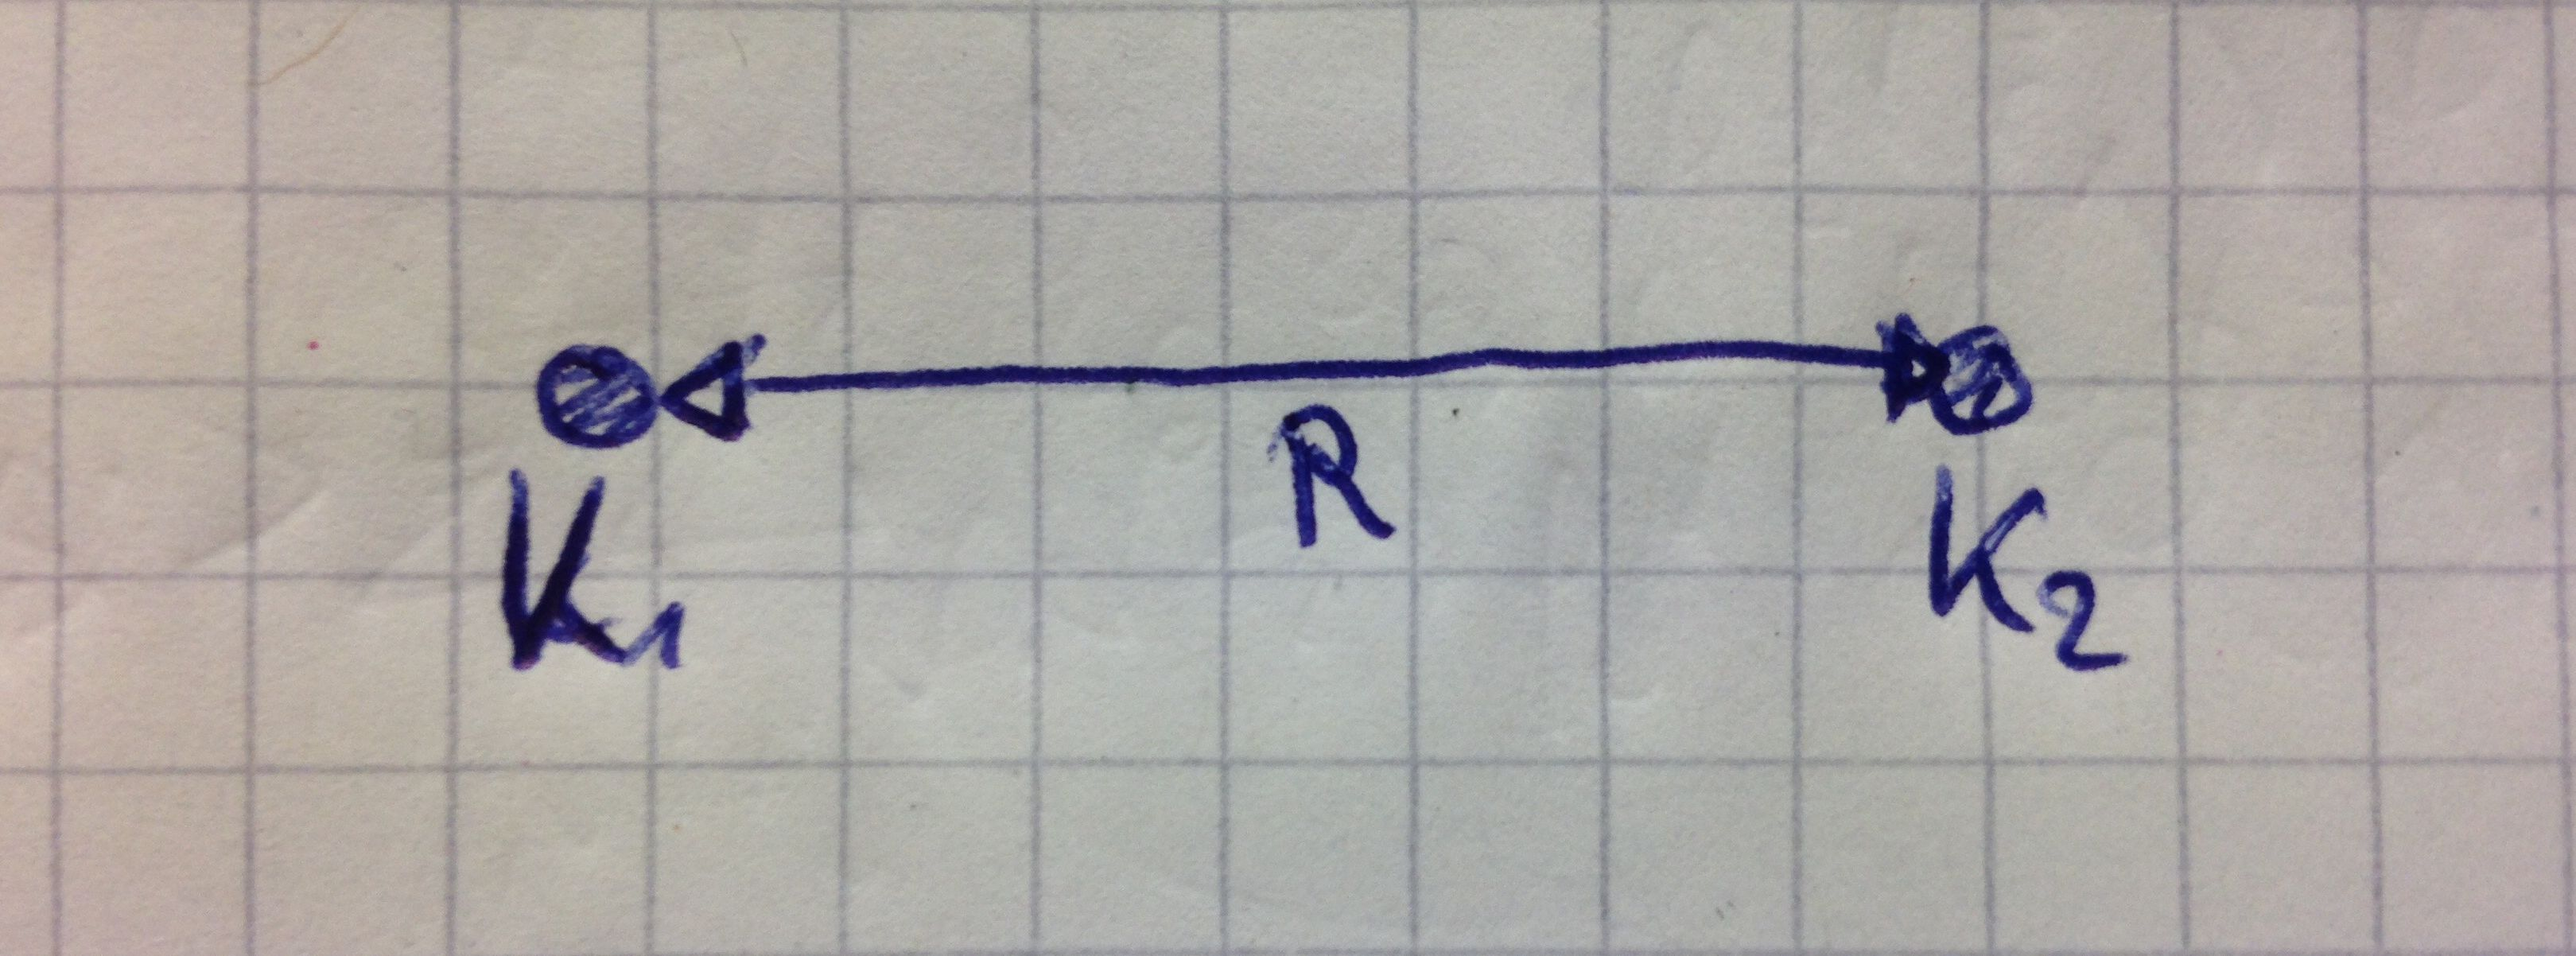
\includegraphics[width=10cm]{Born-Oppenh_Approx1}
				\end{center}
			\end{figure*}
			
		Potenzielle Energie $\U (R)$
			\clearpage
			\begin{figure*} [h]
				\begin{center}
					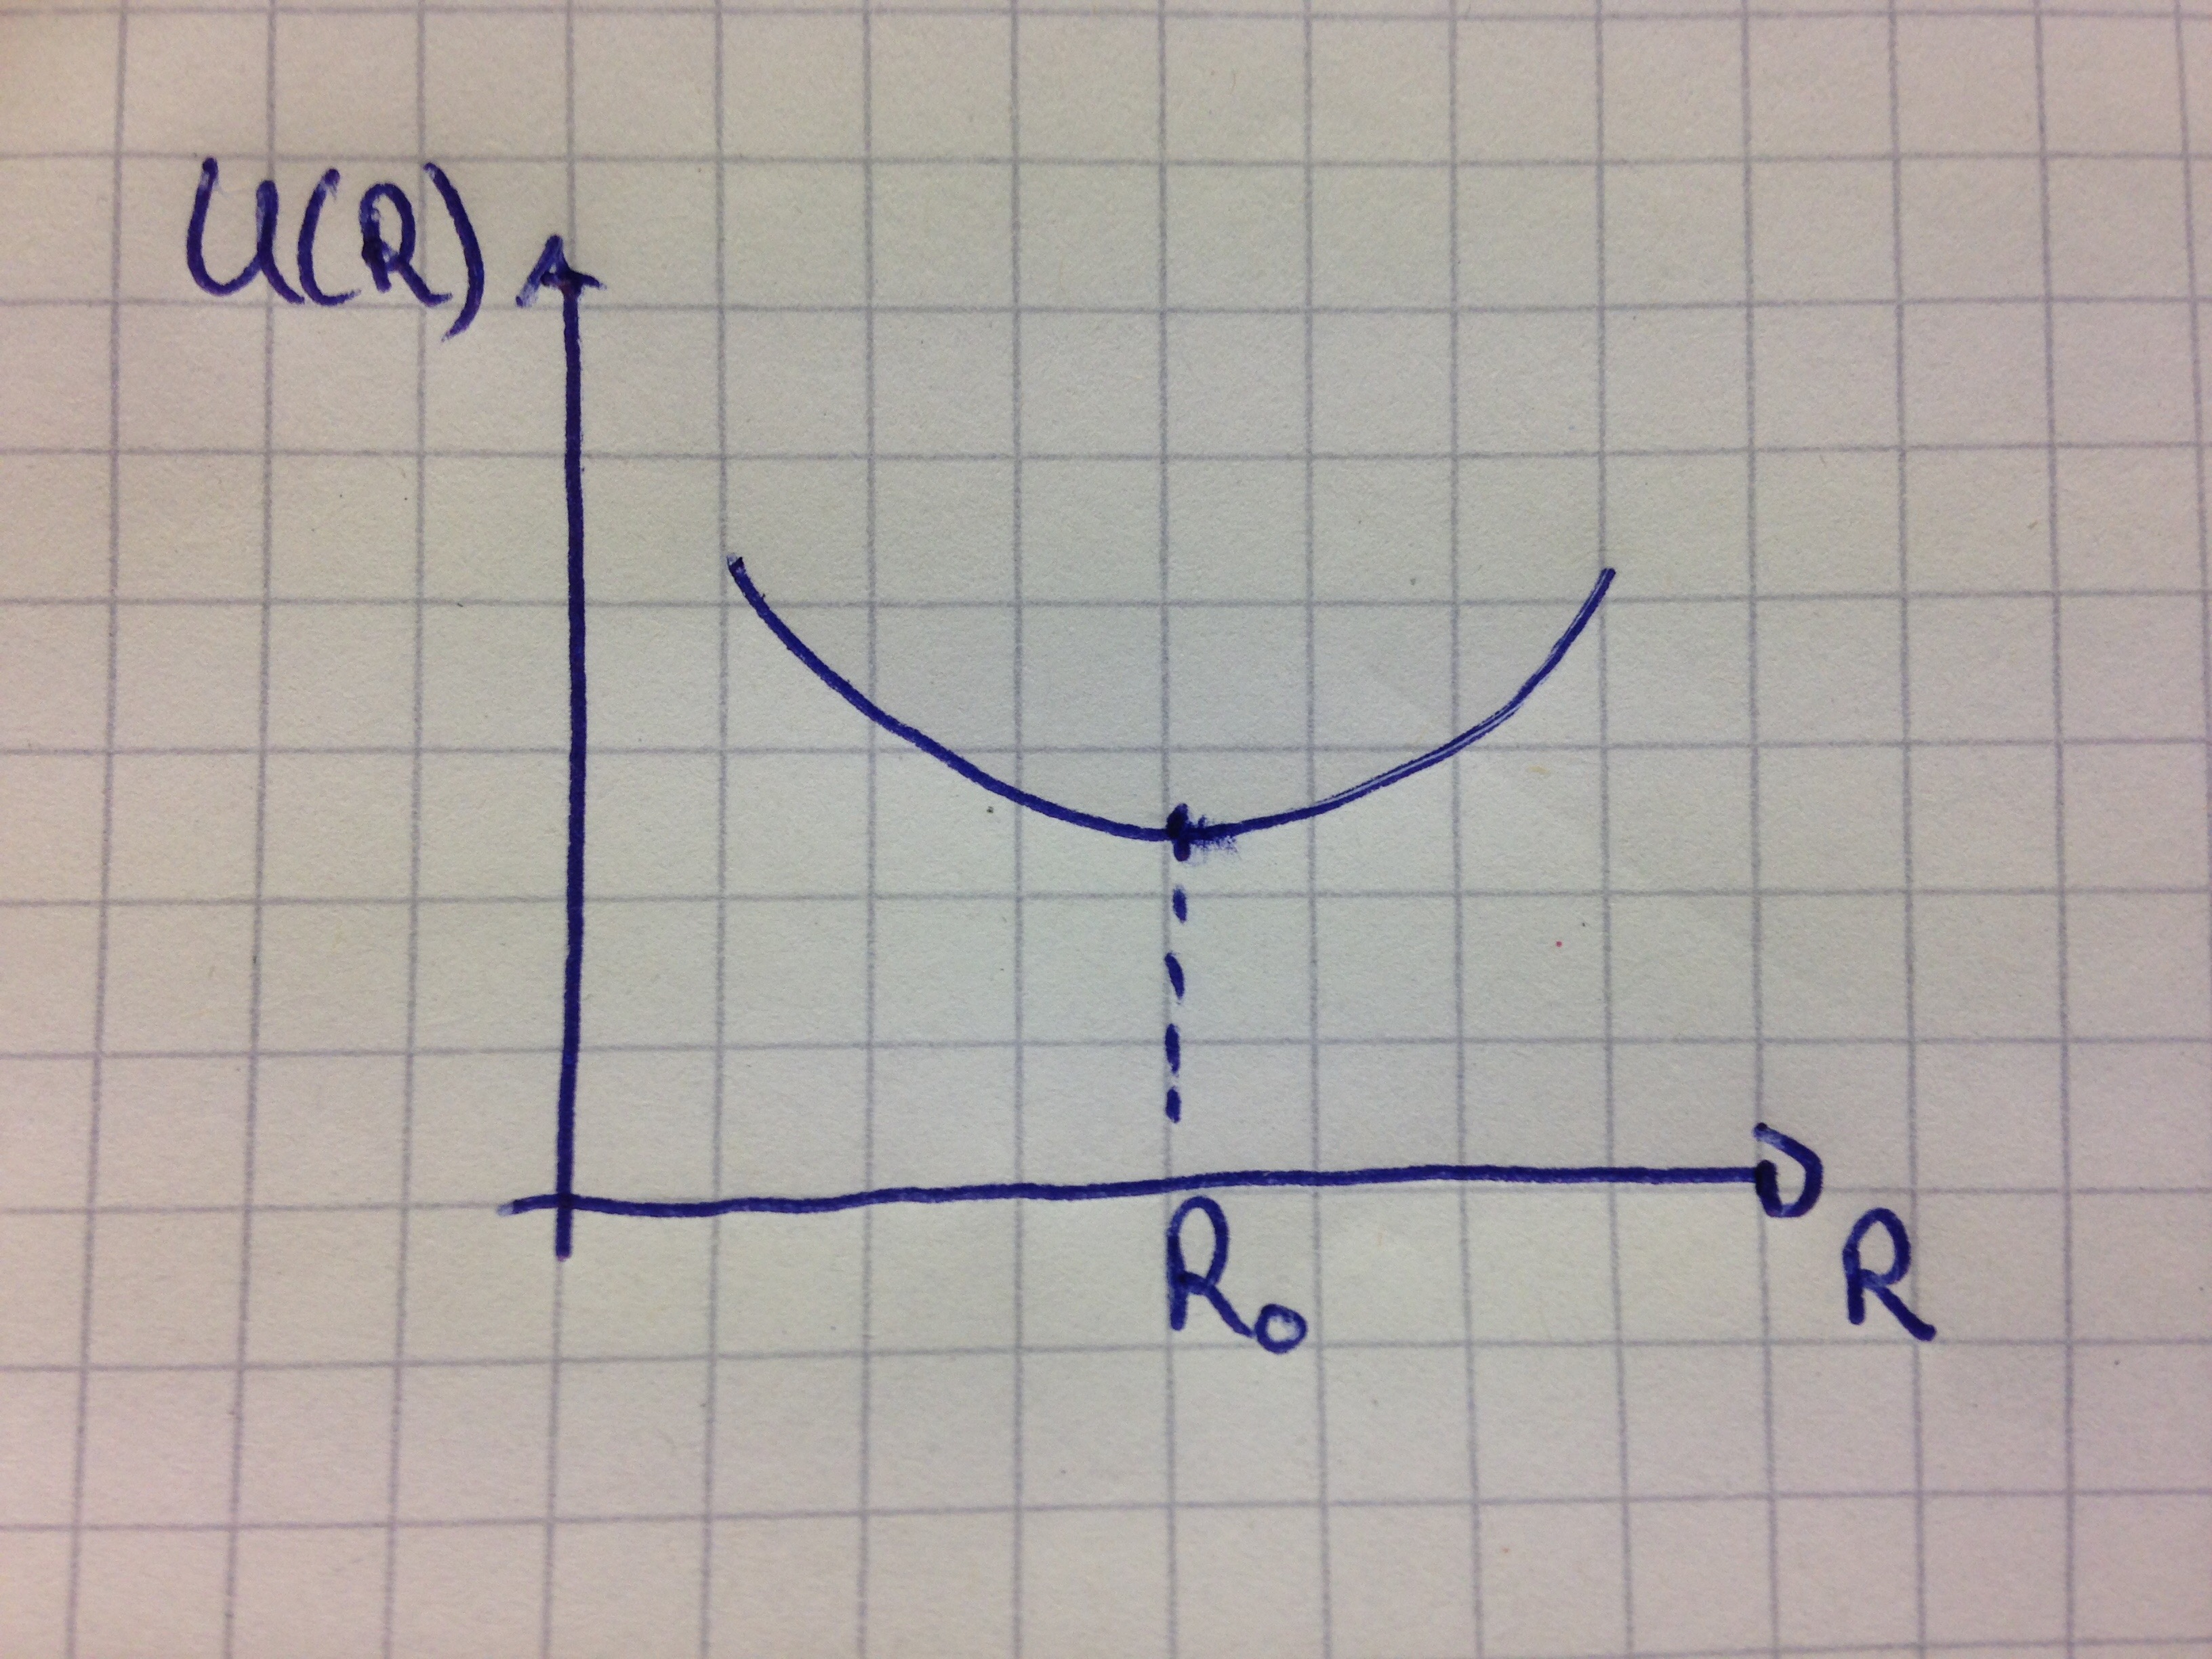
\includegraphics[width=10cm]{Born-Oppenh_Approx2}
				\end{center}
			\end{figure*}
			\begin{align*}
				\U(R) &= const. + \frac{1}{2} m \omega_{\mathrm{vib}}^2 
				\overbrace{(R-R_0)^2}^{\mathclap{< a^2}} \\
				m \omega_{\mathrm{vib}}^2 a^2 &\sim E_{\mathrm{Bindung}} \sim E_{e^-} \\
				E_{\mathrm{vib}} &= \hbar \omega_{\mathrm{vib}} 
				\sim \sqrt{\frac{E_{\mathrm{Bindung}}}{m}} \sqrt{\frac{\hbar^2}{a^2}}
				\sim E_{e^-} \sqrt{\frac{m_e}{m}} \\
				m &\approx 10^4 m_e 
				\Rightarrow E_{\mathrm{vib}} \sim 10^{-2} E_{e^-} 
				\Rightarrow \lambda > 40 \mu \mathrm{m} = 4 \cdot 10^{-3} \mathrm{cm}
			\end{align*}
	\item \underline{Rotationsniveaus}
	
		Trägheitsmoment $I \sim m a^2$
			\begin{align*}
			E_{\mathrm{rot}} &= \frac{L^2}{2 I} 
			= \frac{\hbar^2 \ell (\ell + 1)}{2 I} \sim \frac{\hbar^2}{m a^2}
			\sim \frac{m_e}{m} \cdot E_{e^-} \sim \sqrt{\frac{m_e}{m}} E_{\mathrm{vib}}\\
			&\approx 10^{-4} E_{e^-} \approx 10^{-2} E_{\mathrm{vib}} \\
			\lambda &\approx 0,1 \ldots 1 \mathrm{cm} \\
			&(\omega = 2,45 \mathrm{GHz} \cdot 2 \pi \Rightarrow \lambda \approx 12 \mathrm{cm})
			\end{align*}
		Separation nach Potenz von $\sqrt{\frac{m_e}{m}} \approx \frac{1}{100}$
	\end{enumerate}
	Born-Oppenheimer Näherung:
	
	Elektronische Anregungen beeinflussen kaum die Vibration. Vibrationen beeinflussen kaum den Rotationszustand. 
	$V_{\mathrm{Kern}} \ll V_{e^-}$:
	\begin{enumerate}[1.]
		\item Löse Schrödingergleichung für $e^-$ für gegebenes $R$
		
			Energien (Molekülterme) : $\U_n(R)$
		\item Löse für vorgegebenes $e^-$ Zustand $n$ die Schrödingergleichung: \label{bla}
				\begin{align*}
					\left( - \frac{\hbar^2}{m} \vec{\nabla}_R^2 + \U_n (R)
					\right)	
					\Psi_N (\vec{R}) &= E_N (\vec{R}) \\
					\U_n (R) &\approx const. + \left.\frac{1}{2} \frac{\partial^2}{\partial R^2}
					\right|_{R=R_0} + \ldots = \\
					&= const. + \frac{1}{2} m \omega_{\mathrm{vib}}^2 (R=R_0)^2 
				\end{align*}
			$\Rightarrow$ Schwingungsniveaus: Aufspaltungen: $\mathscr{O} \left(\sqrt{\frac{m_e}{m}}\right)$ unterdrückt
			
			Rotationsmoden: Aufspaltungen $\mathscr{O} \left(\frac{m_e}{m}\right)$
			
		\item Korrigiere $e^-$ Wellenfunktion und $\U_n(R) \curvearrowright \U_{n,N}(R)$ 
			 $\mathscr{O} \left(\frac{m_e}{m}\right)^{\frac{3}{2}}$ 
			 
			 und zurück nach \ref{bla}
	\end{enumerate}
\subsection{Homonukleare Moleküle (Beispiel $H_2$)}
	\begin{figure*} [h]
		\begin{center}
			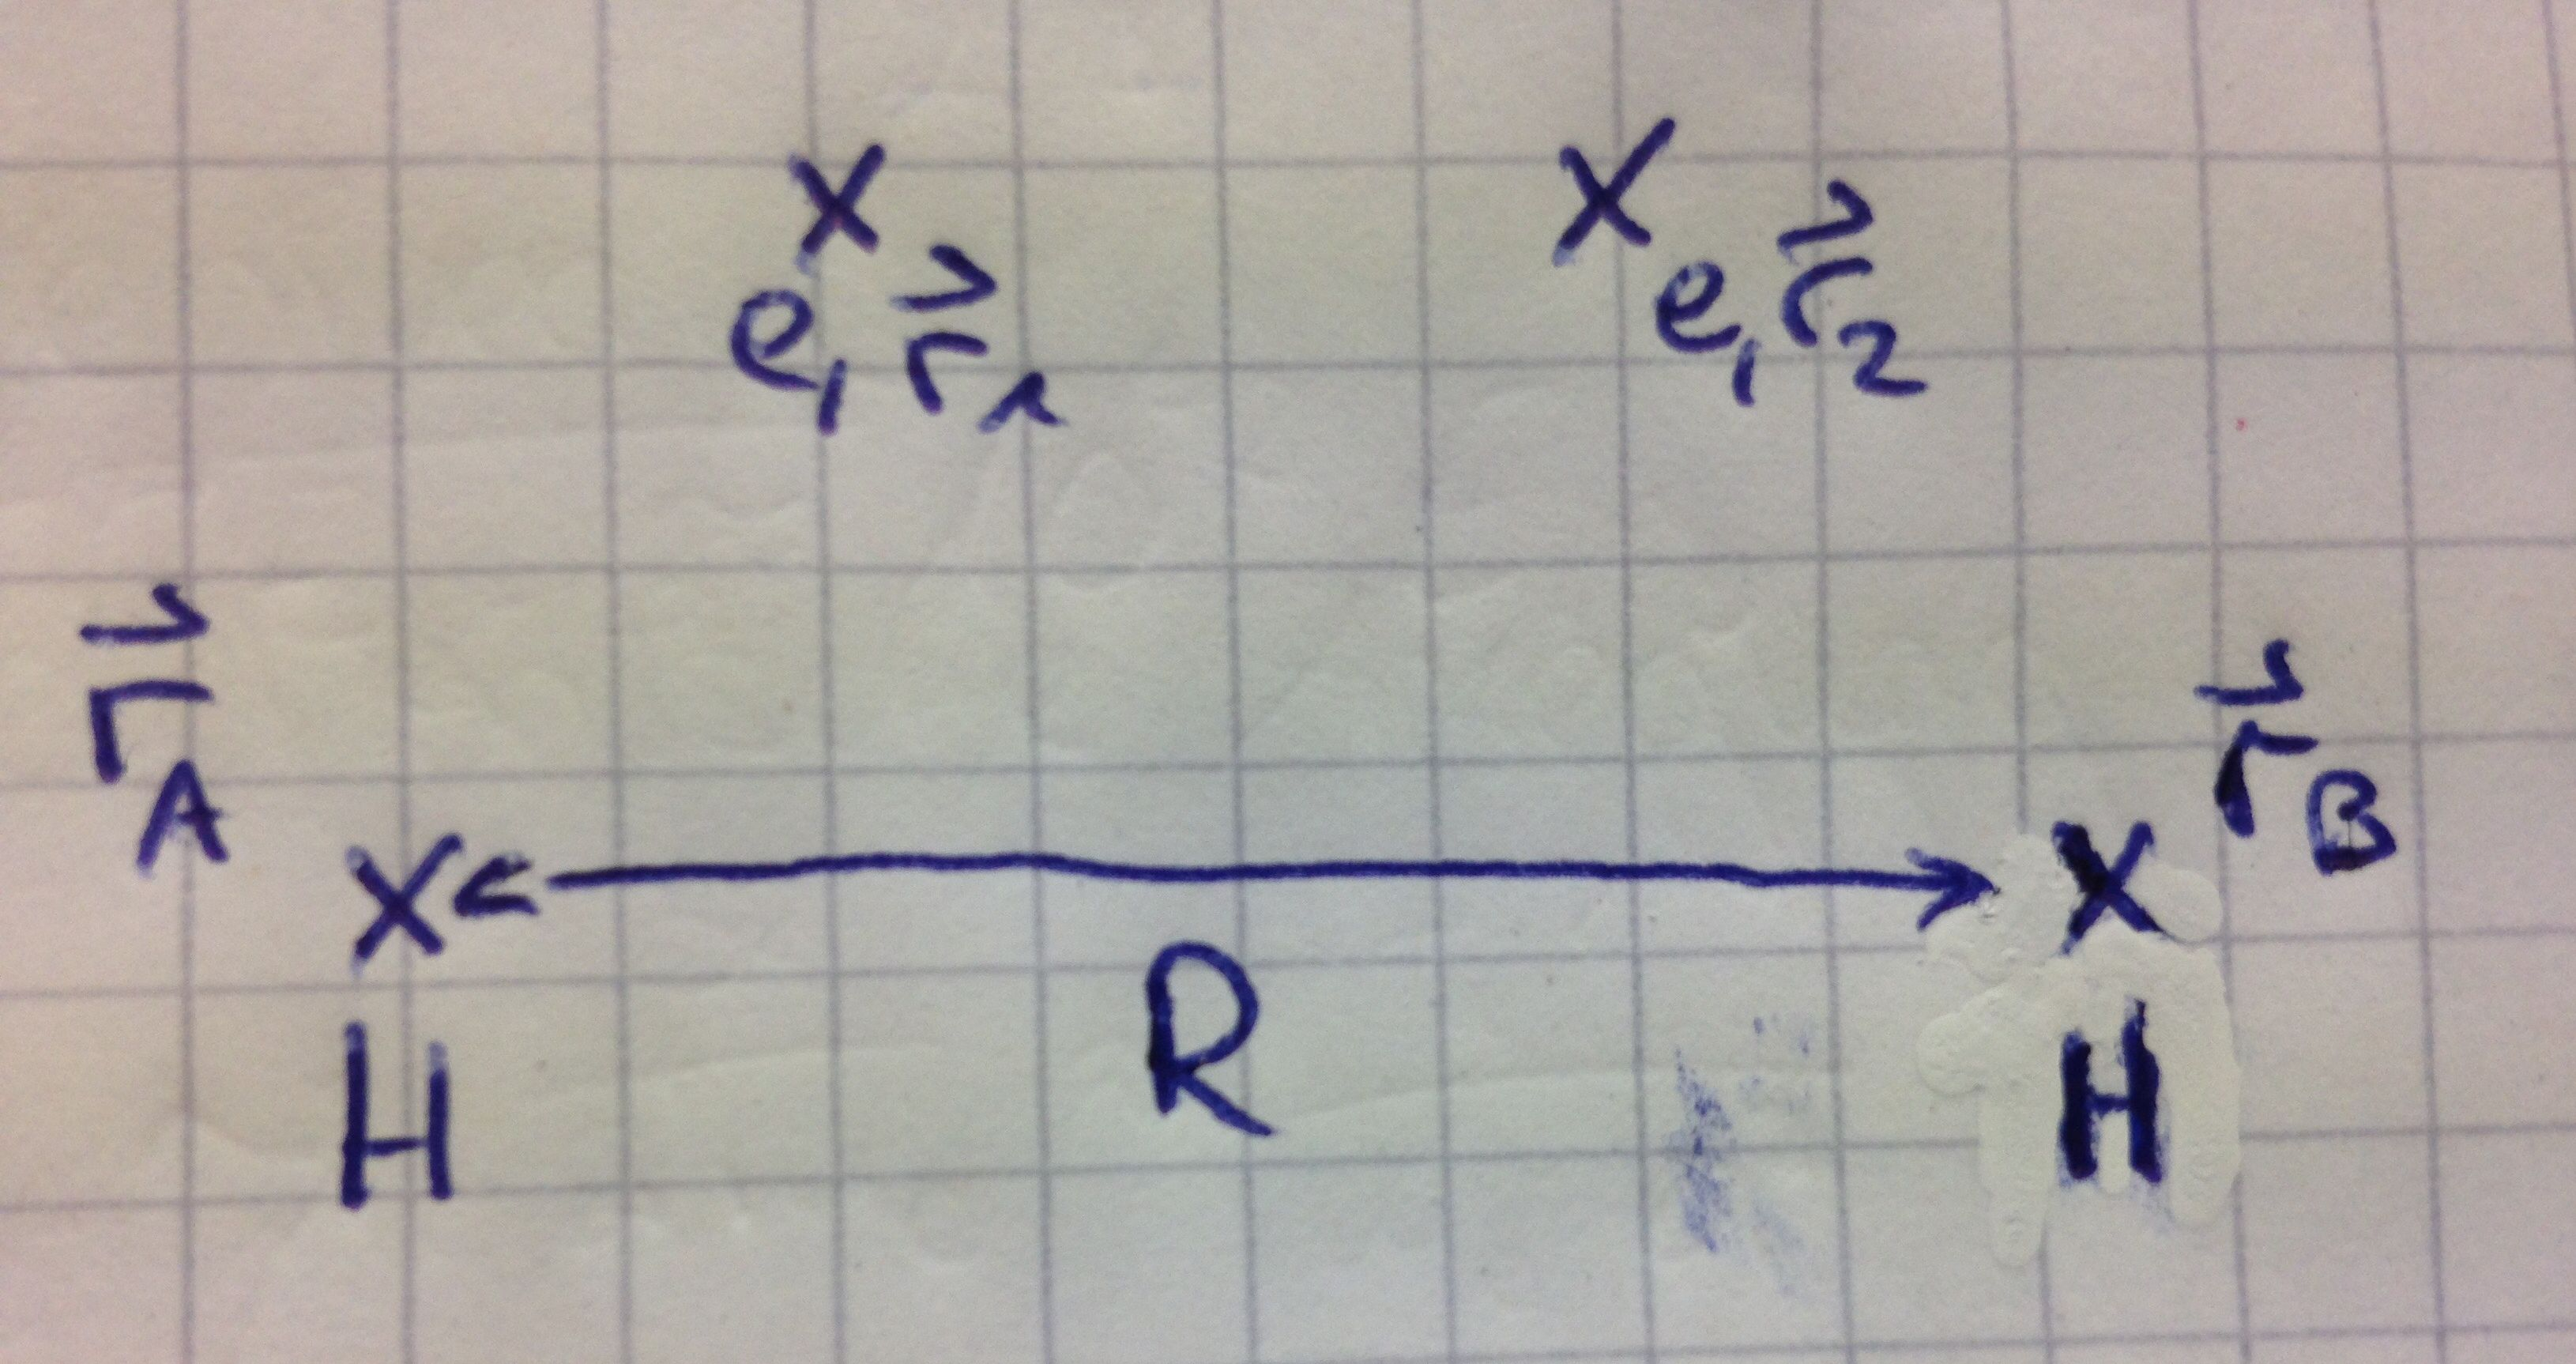
\includegraphics[width=10cm]{Born-Oppenh_Approx3}
		\end{center}
	\end{figure*}